\section{Our process}
Our process was inspired from Essence, which is previously described in \autoref{sec:essence}.
Previous semesters we have been working from a highly Scrum inspired process, but we decided that we wanted to try a new organization this semester.
However, we have chosen to keep sprints, stand-up meetings and retrospective meetings from Scrum as these can compliment Essence.


\subsection{Roles}
We have divided the roles that we described in \autoref{sec:team-organization} between the group.
One person has the role as a \textit{Challenger}.
This person is accountable for prioritizing the tasks we have in our backlog.
The process of prioritizing tasks are further described in the following section.
Another person has the role as \textit{Anchor}.
This person is responsible for changes the process and is in charge of leading evaluations of the process.
The rest of the group functions as \textit{Responders}
These are the developers of the project.
The role as \textit{Child} is fluctuating between the group.
Everyone has the possibility to add suggestions to improve the idea and give other perspectives on the project.


\subsection{Prioritizing task}
Our board on Jira can be seen on \autoref{fig:to-do-board}.
The left most column is the \textit{suggested} column.
Everyone can make suggestions to tasks that they find useful for the project.
At every stand up meeting, we discuss the newly suggested tasks.
What is discussed is the definition of done, how valuable it is for the project and how time consuming it is.
The priority is then $reward - time$, which is an arbitrary number to indicate how important it is.
\\\\
The Challenger then chooses the most important features from discussed often based on the highest priority, as \textit{Chosen for Development}.
Responders then have the opportunity to take tasks from this column and move it to the next column \textit{In progress}.
When the task has been completed, reviewed and merged into develop, it is moved to \textit{Done}.
\begin{figure}[H]
    \centering
    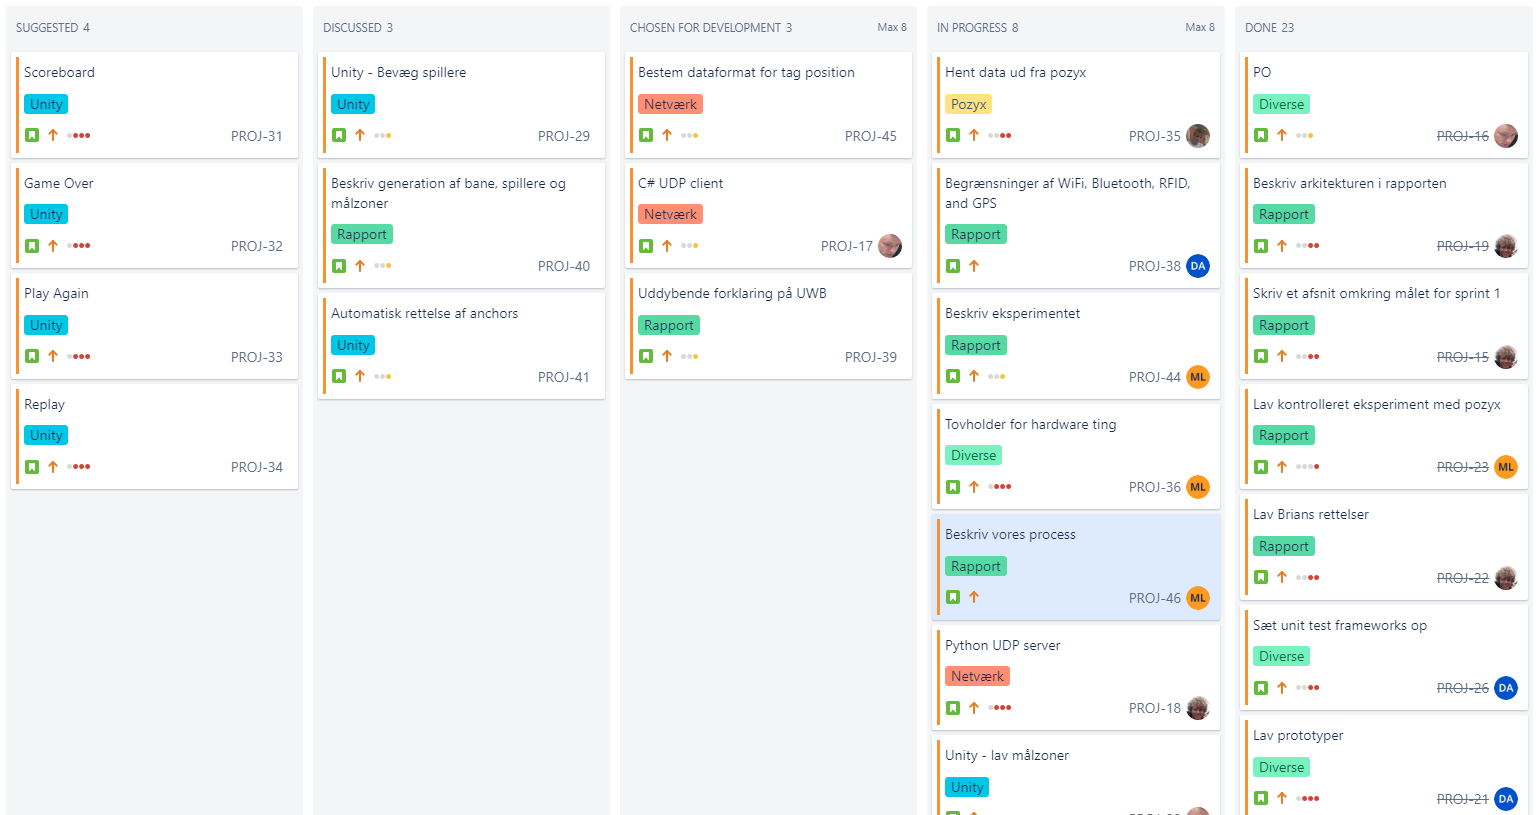
\includegraphics[width=\linewidth]{kanban.PNG}
    \caption{The board for tasks.}
    \label{fig:to-do-board}
\end{figure}

\subsection{Reviews}
Whenever a pull request has been made there are 2 people who 
